%% LaTeX2e class for student theses
%% thesis.tex
%% 
%% Karlsruhe Institute of Technology
%% Institute for Program Structures and Data Organization (IPD)
%% Chair for Software Design and Quality (SDQ)
%%
%% Dr.-Ing. Erik Burger
%% burger@kit.edu
%%
%% Version 1.1, 2014-11-21

%% Available languages: english,ngerman
%% Available modes: draft,final (see README)
\documentclass[english]{sdqthesis}
%% ---------------------------------
%% | Information about the thesis  |
%% ---------------------------------

%% Name of the author
\author{Daniel H. Draper}

%% Title (and possibly subtitle) of the thesis
\title{A Theory of Refinement of Cyber-Physical-Systems into Implementations}

%% Type of the thesis 
\thesistype{Bachelor's Thesis}

%% Change the institute here, ``IPD'' is default
\myinstitute{Institute for Theorethical Informatics}

%% You can put a logo in the ``logos'' directory and include it here
%% instead of the SDQ logo
% \grouplogo{myfile}
%% Alternatively, you can disable the group logo
\nogrouplogo

%% The reviewers are the professors that grade your thesis
\reviewerone{Prof. Dr. Bernhard Beckert}
%\reviewertwo{Prof. B}

%% The advisors are PhDs or Postdocs
\advisorone{Dr. rer. nat. Mattias Ulbrich}
%% The second advisor can be omitted
%\advisortwo{Dipl.-Inform. D}

%% Please enter the start end end time of your thesis
\editingtime{15. April 2015}{15. August 2015}

\settitle

%% --------------------------------
%% | Settings for word separation |
%% --------------------------------

%% Describe separation hints here.
%% For more details, see 
%% http://en.wikibooks.org/wiki/LaTeX/Text_Formatting#Hyphenation
\hyphenation{
% me-ta-mo-del
}

%% --------------------------------
%% | Bibliography                 |
%% --------------------------------

%% Use biber instead of BibTeX, see README
\usepackage[citestyle=numeric,style=numeric,backend=biber]{biblatex}
\usepackage{xr}
\usepackage{listings}
\usepackage{pdfpages}
\addbibresource{thesis.bib}
\newcommand{\keym}{Ke\kern-.2emYmaera}
\newcommand{\key}{Ke\kern-.2emY}


%% ====================================
%% ====================================
%% ||                                ||
%% || Beginning of the main document ||
%% ||                                ||
%% ====================================
%% ====================================
\begin{document}

%% Set PDF metadata
\setpdf

%% Set the title
\maketitle

%% The Preamble begins here
\frontmatter

%% LaTeX2e class for student theses: Declaration of independent work
%% sections/declaration.tex
%% 
%% Karlsruhe Institute of Technology
%% Institute for Program Structures and Data Organization
%% Chair for Software Design and Quality (SDQ)
%%
%% Dr.-Ing. Erik Burger
%% burger@kit.edu
%%
%% Version 1.1, 2014-11-21

\thispagestyle{empty}
\null\vfill
\noindent\hbox to \textwidth{\hrulefill} 
\iflanguage{english}{I declare that I have developed and written the enclosed
thesis completely by myself, and have not used sources or means without
declaration in the text.}%
{Ich versichere wahrheitsgemäß, die Arbeit
selbstständig angefertigt, alle benutzten Hilfsmittel vollständig und genau
angegeben und alles kenntlich gemacht zu haben, was aus Arbeiten anderer
unverändert oder mit Änderungen entnommen wurde.}
 
 
%% ---------------------------------------------
%% | Replace PLACE and DATE with actual values |
%% ---------------------------------------------
\textbf{Karlsruhe, 14th of August, 2015}
\todo{Please replace with actual values}
\vspace{1.5cm}
 
\dotfill\hspace*{8.0cm}\\
\hspace*{2cm}(\theauthor) 
\cleardoublepage

\setcounter{page}{1}
\pagenumbering{roman}

%% ----------------
%% |   Abstract   |
%% ----------------

%% For theses written in English, an abstract both in English
%% and German is mandatory.
%%
%% For theses written in German, a German abstract is sufficient.
%%
%% The text is included from the following files:
%% - sections/abstract

\includeabstract

%% ------------------------
%% |   Table of Contents  |
%% ------------------------
\tableofcontents

\listoffigures
\listoftables

%% -----------------
%% |   Main part   |
%% -----------------

\mainmatter

%% LaTeX2e class for student theses
%% sections/content.tex
%% 
%% Karlsruhe Institute of Technology
%% Institute for Program Structures and Data Organization
%% Chair for Software Design and Quality (SDQ)
%%
%% Dr.-Ing. Erik Burger
%% burger@kit.edu
%%
%% Version 1.1, 2014-11-21

\chapter{Introduction}
\label{ch:Introduction}

The following Bachelorthesis will try to formalize the following process: Replacing the abstract notion of the control program in a verified (by Ke\kern-.2emYmaera) Cyber-Physical-System (\textit{CPS}) with an actual implementation through a form of Formal Refinement and being able to verify that the entire CPS still satisfys the required safety constraints, using both Ke\kern-.2emYmaera and Ke\kern-.2emY. 

CPS are generally modelled as either Hybrid Automata or - Programs.(See ref.~\cite{platzerb}). Mostly, this means, that an abstract version of the discrete control program is modelled, often as a non-deterministic assignment of a control value (See app.~\ref{fig:ex_control}). To replace this non-deterministic assignment with an actual implementation a certain ''glue'' or ''coupling'' has to be found to translate discrete and real continous values into each other. To explain this process we will take a look at the following: 

\begin{enumerate}[label=\bfseries \Roman*:]

\item CPS Watertank (Example taken from Ke\kern-.2emYmaera) refined.
\item Introduction of Formalized used in both examples.
\item CPS Gear-Backlash (See ref.~\cite{bla}) refined.
\end{enumerate}





%% -------------------
%% | Example content |
%% -------------------
\iffalse
\todo{This is the SDQ thesis template.
For more information on the formatting of theses at SDQ, please refer to
\url{https://sdqweb.ipd.kit.edu/wiki/Ausarbeitungshinweise} or to your advisor.

\section{Example: Citation}
\label{sec:Introduction:Citation}
A citation: \cite{becker2008a}

\section{Example: Figures}
\label{sec:Introduction:Figures}
\begin{figure}[h]
\centering

\includegraphics[width=4cm]{logos/sdqlogo}
\caption{SDQ logo}
\label{fig:sdqlogo}
\end{figure}

The SDQ logo is displayed in \autoref{fig:sdqlogo}.

\section{Example: Tables}
\label{sec:Introduction:Tables}
\begin{table}[h]
\centering
\begin{tabular}{r l}
\toprule
abc & def\\
ghi & jkl\\
\midrule
123 & 456\\
789 & 0AB\\
\bottomrule
\end{tabular}
\caption{A table}
\label{tab:atable}
\end{table}

\section{Example: Todo-Note}
Meaningless text.
Replace with meaningful text. (This note is only shown in draft mode.)

\section{Example: Formula}
One of the nice things about the Linux Libertine font is that it comes with
a math mode package.
\begin{displaymath}
f(x)=\Omega(g(x))\ (x\rightarrow\infty)\;\Leftrightarrow\;
\limsup_{x \to \infty} \left|\frac{f(x)}{g(x)}\right|> 0
\end{displaymath}
}
\fi
%% --------------------
%% | /Example content |
%% --------------------
%% LaTeX2e class for student theses
%% sections/preliminary.tex
%% 
%% Karlsruhe Institute of Technology
%% Institute for Program Structures and Data Organization
%% Chair for Software Design and Quality (SDQ)
%%
%% Dr.-Ing. Erik Burger
%% burger@kit.edu
%%
%% Version 1.1, 2014-11-21


\chapter{Preliminary Definitions}
\label{ch:Preliminary}

In the following chapter we want to define and explain terms, models and logic used throughout this thesis. We skip the explanation of first-order logic, which we presume to be known by the reader.

\section{Introducing Cyber-Physical Systems}
\label{sec:pre:cps}

In this thesis we take a close look at \textbf{Cyber-Physical Systems}. These are systems in which a physical aspect or value is controlled by a computer (program). For example, an aircraft control system in which the computer exerts a form of speed control on the airplane would be a CPS. 

For our purposes we also refer to CPS as \textit{Hybrid Systems}, in which discrete values (in the control program) and continuous values (in the physical world) coexist. The difficulty in analyzing these kinds of systems stems from the ``hybridness'' of the systems: There is always some form of translation necessary to go from the program (discrete values) world to the physical (continuous reals) world. 

\subsection{Modeling CPS as Hybrid Automata}

Two different modeling approaches exist for CPS, the first one we now explain are hybrid automata. Formally they are defined to have the following components (From~\cite{Heinzinger2000b}):
\begin{quote}
		\begin{description}
			\item[\textit{Variables}]A finite set \(X = \{x_1,\dots , x_n\}\) of real numbered variables. The number \(n\) is called the dimension of \(H\). [...]
			\item[\textit{Control graph}]A finite directed multigraph \((V, E)\). The vertices in \(V\) are called control modes. The edges in \(E\) are called control switches.
			\item[\textit{Initial, invariant, and flow conditions.}]Three vertex labeling functions \(init\), \(inv\) and \(flow\) that assign to each control mode \(v\in V\) three predicates. [...]
			\item[\textit{Jump conditions}]An Edge labeling function jump that assigns to each control switch  \(e \in E\) a predicate.
			\item[\textit{Events}]A finite set \(\Sigma\) of events, and an edge labeling function event: \(E \rightarrow \Sigma\) that assigns to each control switch an event.
		\end{description}
\end{quote} 

Based on non-deterministic finite automata (NFA), they are easy to understand for humans and serve well to model the abstract behavior of hybrid systems. A possible hybrid automata can be seen in Fig.~\ref{fig:automata}. It describes the behavior of a controller controlling the train on a rail section. A train is therefore always either traveling freely (accelerating)  or being slowed. The biggest difference to NFAs is apparent when looking inside both states: They are continuous, so there is no single value assigned to the train's acceleration but rather a description of the behavior of the value over time is given. This means, that the single state "accelerate" can also be seen as a continuous flowing assignment of values according to the specified differential equation.~\cite{platzer2010b}.

The system still obviously exhibits its continuous behavior, as any change to the acceleration also brings the change of speed and location. As the train passes the arbitrarily chosen point \emph{SB}, the controller automatically assigns a discrete negative value to the train's acceleration, decelerating it, so it slows down. In the brake state the train again follows the equations of linear motion with continuous assignment, only that the guard \(v \geq 0\) makes sure the train never travels backwards (with a negative velocity), but rather at some point starts accelerating again according to the discrete assignment in the state change between brake and accelerate.

\begin{figure}[ht!]
	\centering
	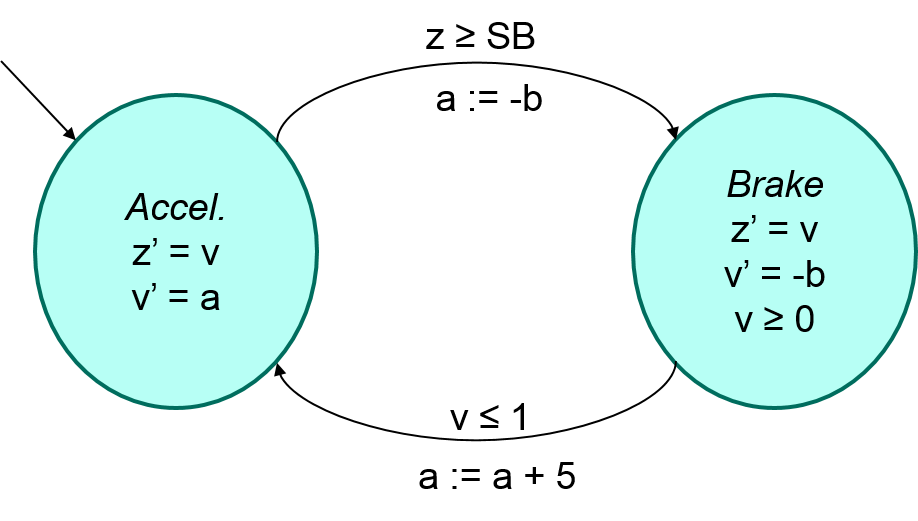
\includegraphics[width=1.0\textwidth]{images/automata}
	\caption{A simple Hybrid Automata~\cite{platzer2010b}.}
	\label{fig:automata}
\end{figure}

\subsection{Modeling CPS as Hybrid Programs}

As we are using \keym~for verification, which uses Hybrid Programs (HP), we also have to introduce the syntax of hybrid programs. They follow the syntax depicted in table~\ref{tab:hp}, whereby \(\theta_i\) are terms, \(x_i \in \Sigma\) are state variables and \(\chi\) is a formula of first-order logic~\cite{platzer2010b}.

As an example we take a look at the hybrid program notation of a train control system (See Fig.~\ref{fig:etcs_hp}). As can be seen, the state variable \(x\) is first assigned the state accelerate, this corresponds to the hybrid automaton's (See Fig.~\ref{fig:automata}) starting state. In line 3 we can see the hybrid program syntax being an extension of first-order logic: Only if \(q=accel\) \textbf{and} \(z \geq SB\) are true can this case be enacted (corresponding to the state change from accel. to brake in the automaton).

\begin{table}
	\begin{tabular}{p{5cm} | p{4cm} | p{6cm} }
		notation & statement & effect \\ \hline
		\(x := \theta\) & discrete assignment & assigns term \(\theta\) to variable \(x\) \(\in\) \(V\) \\
		\(x := \ast\) & nondet. assignment & assigns any real value to \(x \in V\) \\
		\(x^{\prime}_1 = \theta_1 \wedge ... \newline
		... \wedge x^{\prime}_n = \theta_n \wedge \chi\) & continuous evolution & diff. equations for \(x_i \in V\) and terms \(\theta_i\),\newline
		with formula \(\chi\) as evolution domain \\
		\(?\chi\) & state check & test formula \(\chi\) at current state \\
		\(\alpha;\beta\) & seq. composition & HP \(\beta\) starts after HP \(\alpha\) finishes \\
		\(\alpha \cup \beta\) & nondet. choice & choice between alternatives HP \(\alpha\) or \(\beta\) \\
		\(\alpha^\ast\) & nondet. repetition & repeats HP \(\alpha\) \(n\)-times for any \(n \in \mathbb{N}\) \\
		%\it{do} \(\alpha\) \it{until} \(\chi\) & evolve until &  evolve HP \(\alpha\) until \(\chi\) holds \\
	\end{tabular}
	\caption{Syntax of Hybrid Programs (HP)~\cite{platzer2010b}.}
	\label{tab:hp}
\end{table}

\begin{figure}[ht!]
	\(q := accel;\)\newline
	\(((?q = accel; z^{\prime}= v, v^{\prime}= a)\) \newline
	\(\cup~(?q = accel \wedge z \geq SB; a := -b, q:= brake; ?v \geq 0)\) \newline
	\(\cup~(?q = brake; z^{\prime}=v, v^{\prime}= -b ~ \& ~ v \geq 0)\) \newline
	\(\cup~(?q = brake \wedge v \leq 1; a := a+5; q := accel))^\ast\)
	\caption{A simplified train control system as a Hybrid Program~\cite{platzer2010b}.}
	\label{fig:etcs_hp}
\end{figure}

\section{Dynamic Logic}
\label{sec:pre:DL}

Dynamic logic is a multi-modal logic and has two basic operators (one of which is relevant to this thesis): Either \textit{safety} (\([]\)) in which a first-order-logic formula \(\phi\) holds true in all exit states of the program \(\alpha\). Or \textit{liveness} (\(\langle\rangle\)), where a possible execution of the program \(\alpha\) exists, after which the first-order-logic formula \(\phi\) holds. In this paper only the safety operator is used. The operators can be expressed as in Eq.~\ref{eq:ddl}, whereby \(\alpha\) denotes the (hybrid) program that is enacted, and \(\phi\) is the postcondition expressed in first-order-logic.

\begin{equation}
	\begin{split}
		\mathit{Safety}: [\alpha]\phi \\
		Liveliness: \langle\alpha\rangle\phi \equiv \neg ([\alpha] \neg \phi) \\
	\end{split}
	\label{eq:ddl}
\end{equation}

\subsection{Differential Dynamic Logic}
\label{subsec:DDL}

As dynamic logic in itself was not specifically devised for hybrid programs, this means we need a way to express differential equations, as most continuous movement or behavior is expressed by differential equations. DDL or d\(\mathcal{L}\), the language also used by our verification tool \keym, has ways to express differential equations, as can be seen in Table~\ref{tab:hp}. d\(\mathcal{L}\) is a \begin{quote} ``free variable proof calculus [...] with a [...] combination of real-valued free variables and Skolemisation for lifting quantifier elimination for real arithmetic to dynamic logic''~\cite{PlatzerDl}.\end{quote}

The d\(\mathcal{L}\) formulas use the syntax from Table~\ref{tab:hp}, and are defined as in first-order dynamic logic, using the operators described in the previous section, propositional connectives (\(\neg, \wedge, \vee, \implies, \iff\)), as well as quantifiers (\(\forall, \exists\)).

\subsection{JML: Verification of Java Programs using \key}
\label{subsec:jml}

In this thesis we also deal with the verification of Java programs (the control programs of our cps). We now want to introduce the Java Modeling Language \textit{JML}, which is used to model specification of Java classes/modules or single methods. JML is based on the Design-By-Contract premise, which means that the user and the Java classes have a contract with each other which defines the input and output conditions of the program~\cite{keybook2007}. JML is then listed as a comment in the Java source code right before the method in question~\cite{fmcoKeYTutorial06}. For example the JML code for a method in question could look like this:


\definecolor{darkgreen}{rgb}{0.0, 0.2, 0.13}
\lstset{language=Java,captionpos=b,tabsize=3,frame=lines,keywordstyle=\color{blue},commentstyle=\color{darkgreen},stringstyle=\color{red},numbers=left,numberstyle=\tiny,numbersep=5pt,breaklines=true,showstringspaces=false,basicstyle=\footnotesize,emph={label}}
\begin{lstlisting}[label=lst:jml_example]

/*@ public normal_behavior
  @ requires a >= 0
  @ ensures b >= 2
  */
  public int getPlusTwo(int a) {
  	b = a + 2;
  	return b;
}

\end{lstlisting}

As one can see, the JML contract needs to have an access level and (for our purposes) always will have a \textit{requires} precondition that must hold true before the method is called for all arguments or some class variables and a \textit{ensures} postcondition clause, that has to hold true for all exit states of the method (where the precondition was true before calling it). This means the JML contract above produces the proof obligation below:

\begin{equation}
	a \geq 0 \implies [b = getPlusTwo(a) ] b \geq 2
	\label{eq:jmlddl}
\end{equation}

\subsection{Java Dynamic Logic}
\label{subsec:jdl}

Internally, \key~translates the contract specified in JML into its own dynamic logic form, Java Card Dynamic Logic. It is a multi-modal logic, that makes the formulation of statements about the program behavior possible. Therefore it combines Java programs and dynamic formulas in a single language. It is based on first-order Dynamic logic as is DDL and can be seen as an extension of Hoare Logic. While a proof obligation \(\alpha[p]\beta\) is similar to the Hoare triple \(\{\alpha\}p\{\beta\}\), in JDL, \(\alpha\) and \(\beta\) both can contain further programs, while in Hoare Logic they are strictly first-order formulas~\cite{keybook2007}.

\section{\keym~as our Verification Tool for Hybrid Programs}
\label{sec:pre:key}

As \key~can only deal with Java programs, but we deal with problems with hybrid systems, we use \keym~as our tool of choice to verify our hybrid models. It is based on \key's source and developed by Andr\'e Platzer at Carnegie Mellon University~\cite{keymaera}. As its back-end arithmetic solver we used Wolfram Mathematica~\cite{mathematica}, but \keym~supports other computer algebra solvers as well. For verification of our glue relation we also express the problem in a hybrid program form, and use \keym~as our automatic solver.

Hybrid Programs are expressed as \textit{regular programs}, but as for example \(\cup\) is not a symbol used in ASCII text, the program notation in the \textit{.key} \keym-files is different (e.g. \(\cup\) as \(++\)), but we will present every hybrid program in the syntax presented above as well as to avoid confusion and adding another layer of abstraction.

%% LaTeX2e class for student theses
%% sections/content.tex
%% 
%% Karlsruhe Institute of Technology
%% Institute for Program Structures and Data Organization
%% Chair for Software Design and Quality (SDQ)
%%
%% Dr.-Ing. Erik Burger
%% burger@kit.edu
%%
%% Version 1.1, 2014-11-21

%To be able to reference labels in other file
\externaldocument{introduction}

%%%%%%%%%%%%%%%%%%%%%%%%%%%%%%%%%%%%%%%%%%%%%%%%%%%%%%%%%%%%%%%%%%%%%
%--WATERTANK--%
%%%%%%%%%%%%%%%%%%%%%%%%%%%%%%%%%%%%%%%%%%%%%%%%%%%%%%%%%%%%%%%%%%%%%
\chapter{Example-based Refinement on CPS Watertank}
\label{ch:Watertank}

To get a better understanding of the tasks involved in refining a hybrid model into a implementation with all necessary intermediate verification steps, we took a look at one of the out-of-the-box examples provided in the \keym~tutorial~\cite{keYmaera}, a Watertank (See fig.~\ref{fig:watertank}).

\begin{figure}
	\setcounter{figure}{0}
	\centering
	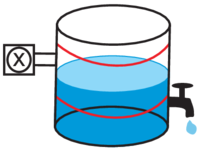
\includegraphics[width=0.6\textwidth]{images/watertank}
	\caption{Picture of possible Watertank configuration: Watertank that can get drained at all times and has a valve controlled by a control program~\cite{keymaeraGuide}.}
	\label{fig:watertank}
\end{figure}

The ``control'' part of this hybrid system is the valve, it can either drain the watertank with a rate of \(-2\) or it can fill the tank further with a rate of \(1\). The goal of the entire system then is, to keep the water level \(y\) of the tank between \(1\) and \(12\). Normally this is proven by \keym~ without actually implementing a control program. As our goal is to find a concrete implementation,  we first took a look at the hybrid model of the watertank. It is provided both in the form of a hybrid automata (See fig.~\ref{fig:watertank_ha}) and a hybrid program (See fig.~\ref{fig:watertank_hp}).

\begin{figure}
	\centering
	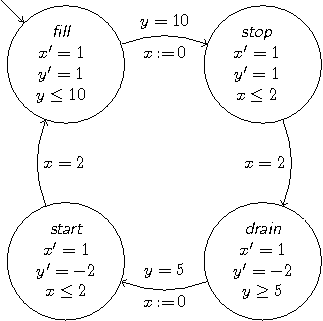
\includegraphics[width=0.6\textwidth]{images/watertank_ha}
	\caption{The Watertank CPS expressed as a hybrid automata~\cite{keymaeraGuide}.}
	\label{fig:watertank_ha}
\end{figure}

\begin{figure}
	\centering
	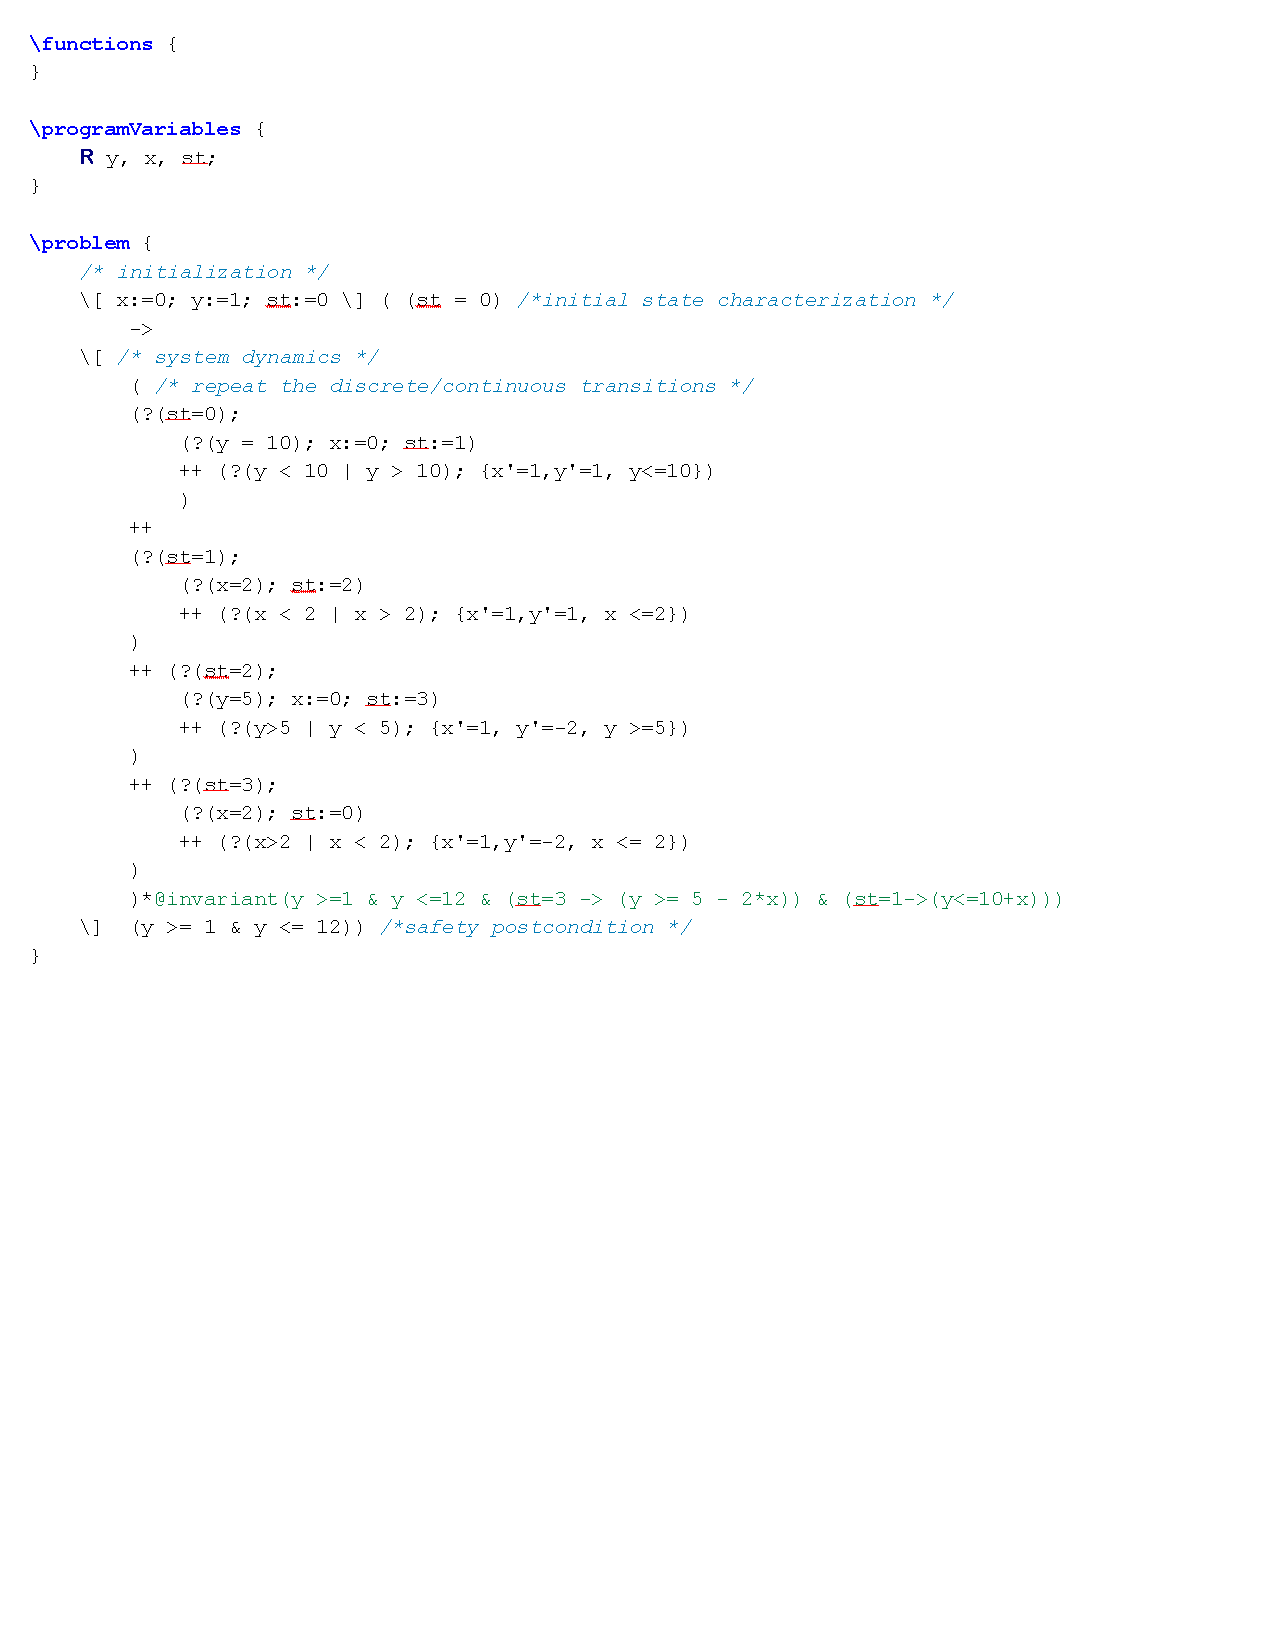
\includegraphics[width=0.8\textwidth]{images/watertank_hp}
	\caption{The Watertank CPS expressed as a hybrid program~\cite{keymaeraGuide}.}
	\label{fig:watertank_hp}
\end{figure}

\section{Finding the concrete Control Value Assisgnment}
\label{sec:Watertank:ControlValue}

In order to be able to apply Eq.~\ref{eq:Main_LogicRefinement} to this concrete example, the first challenge we faced was finding a spot in which a (or multiple) concrete control value is actually assigned. We call this assignment(s) the \textit{hook} as the actual implementation will ``hook'' into our hybrid model at this exact point. Taking a look at the Hybrid Automata describing the Watertank (See fig.~\ref{fig:watertank_ha}), it became obvious, that the hybrid model of the watertank required changing to be able to find our actual ``hook''. In the original model, a control value is never explicitly assigned, rather does the valve change its state non-deterministically, making a deterministical control program implementation impossible. Therefore, we tried to remodel the model to better serve our purpose, featuring a clear ticked hook that is called upon at deterministic times. (See fig.~\ref{fig:watertank_hp_ref}).

\begin{figure}
	\centering
	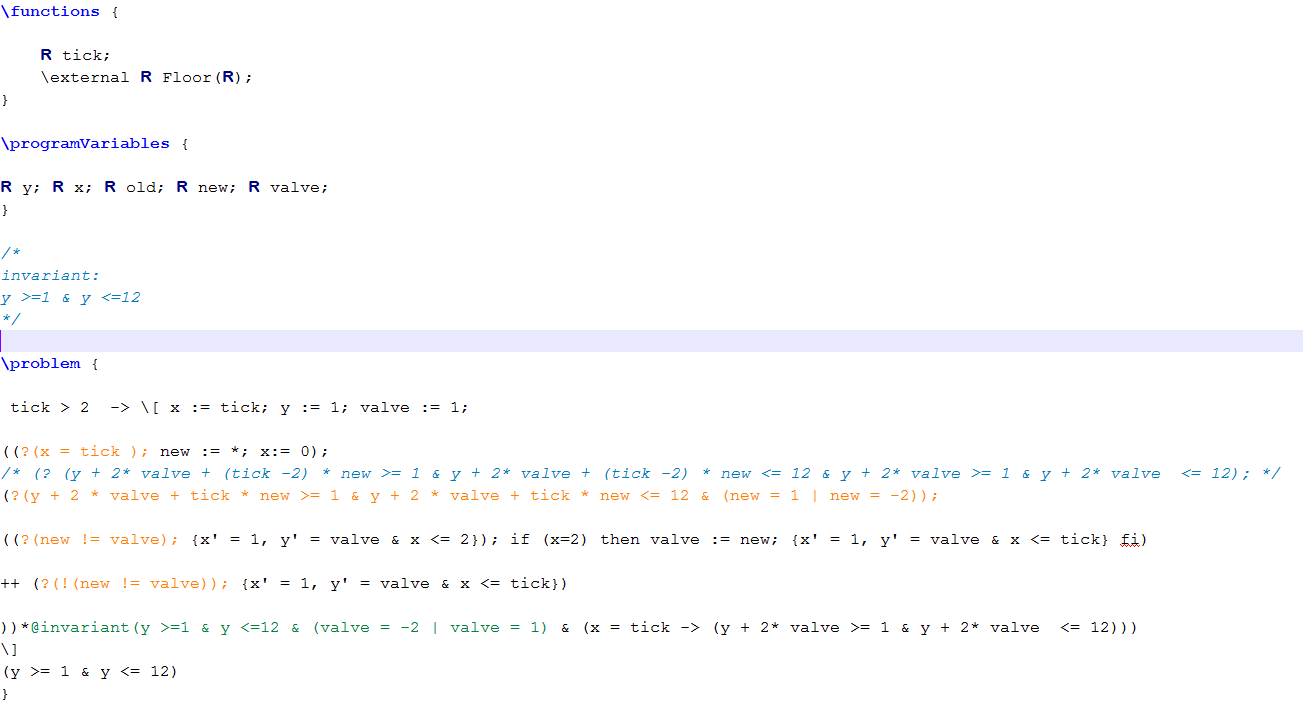
\includegraphics[width=0.9\textwidth]{images/watertank_hp_ref}
	\caption{The Watertank CPS after remodelling to account for hook.}
	\label{fig:watertank_hp_ref}
\end{figure}

We tried to keep the model mostly equivalent to the original, preserving the 2 clock ticks of time needed for the valve to change its state from drain to fill and vice-versa. This then proved difficult, when trying to think of possible implementations, as the program hook could be called again before the valve would have actually changed its state. To simplify this problem, we decided to only model cases in which the actual program tick (so the time between two hook calls)  is greater than 2 clock ticks (however long they may be).  This means, that the valve or control program doesn't have to have a (possibly infinite) list of the last control values assigned, which could be the case if the program was called more frequently than the valve is able to change states.

\section{Refining the original Hybrid Automata}
\label{sec:Watertank:Refinining}

\section{Finding the correct Program Safety Condition}
\label{sec:Watertank:SafetyCond}

The next step we attempted was finding the correct postcondition for the program hook (\(\psi\) in eq.~\ref{eq:Main_LogicRefinement}), which would then serve as the abstraction of the java control program we would later implement. This means, that the program would be built accordingly, so that it could be verified against this postcondition. The original postcondition we devised:

\begin{equation}
	\centering
	\begin{split}
		\psi \equiv ?( y + 2* valve + tick -2 * new  >= 1~\&~ \\ 2 * valve * (tick - 2) * new <= 12~\&~ \\  y + 2* valve >= 1~\&~ y + 2 * valve <= 12) 
	\end{split}
\label{eq:postCondOrig}
\end{equation}

When trying to verify the entire hybrid program (see comment in line 5 of the problem in fig.~\ref{fig:watertank_hp_ref}), this postcondition did not work. This means, that even in such a simple CPS as this watertank control system, finding the hook postcondition was non-trivial and only with the help of \keym's counterexamples did we manage to find the correct postcondition (See eq.~\ref{eq:postCondOrigCorrect}). 

\begin{equation}
	\centering
	\begin{split}
		\psi \equiv (?(y + 2 * valve + tick * new >= 1~\& \\ y + 2 * valve + tick * new <= 12~\& \\(new = 1 | new = -2))
	\end{split}
	\label{eq:postCondOrigCorrect}
\end{equation}

\keym~ verified our new hybrid program fully automatically (See fig.~\ref{fig:KeymaeraVerWatertank}).

\begin{figure}
	\centering
	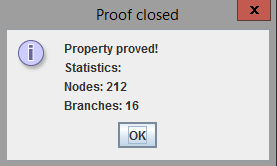
\includegraphics[width=0.6\textwidth]{images/watertank_keym_ver}
	\caption{The result of automatic verification by \keym~ of the Watertank hybrid program that includes our hook (See fig~\ref{fig:watertank_hp_ref}).}
	\label{fig:KeymaeraVerWatertank}
\end{figure}

\section{The (simple) Java Control Program}
\label{sec:Watertank:Java}

After completing verification of our hybrid model with \keym, we proceeded to implement a (simple) control program for the Watertank. Finding a suitable implementation proved difficult, as a parallel implementation (Both the control system and the differential equations working in parallel, modifying the water level) seemed more intuitive. This would defeat the purpose of actually finding a suitable hook and was more based on our understanding of the original hybrid model and not our version including the hook.

Using our understanding of a singular hook of the control system into the Watertank as well as the hook postcondition from the previous section as our specification for the actual control method, that would return the control value to the Watertank's valve, we then managed to implement a suitable discrete control method (See fig.~\ref{fig:source_controlMethod}).

\begin{figure}
	\centering
	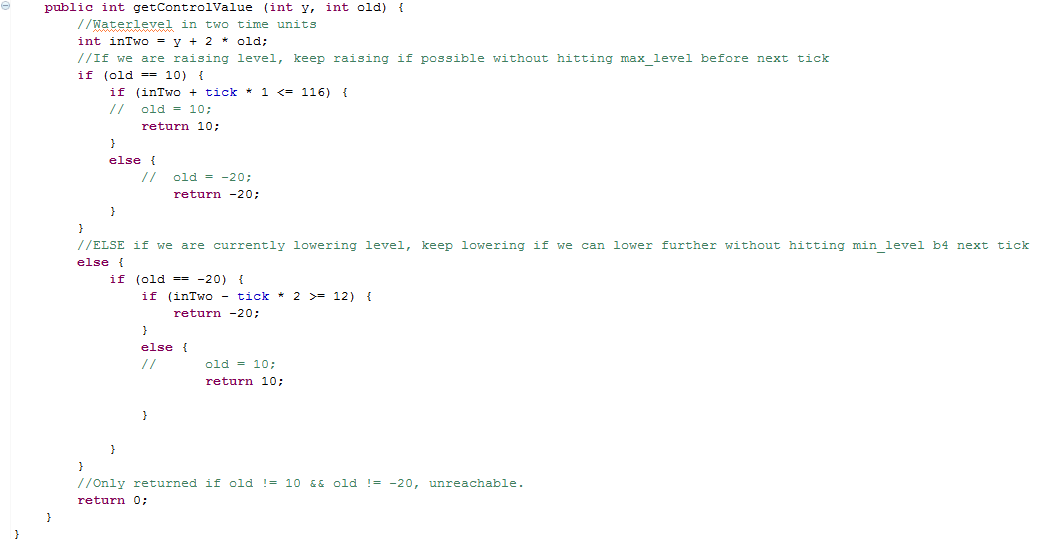
\includegraphics[width=0.9\textwidth]{images/source_control_method}
	\caption{The actual control method implemented.}
	\label{fig:source_controlMethod}
\end{figure}
The control method consists only of simple if-else-statements and just assigns the best-case (keep raising level if we were raising, keep lowering if we are lowering as long as postcondition is still valid) value to the valve.
For testing purposes, we also implemented a complete simulator of the Watertank CPS (See app.~\ref{app:fig:source_sim}).

\section{Finding the glue between Java and the Hybrid Model of the system}
\label{sec:Watertank:Glue}

The most important and also difficult part of our process, was finding the glue between the real parts of the hybrid system and our java control program. As real values (used in the hybrid model) and discrete values (used in our java implementation) are fundamentally different, a certain transformation has to occur.  In the Watertank example, this means, that the waterlevel as well as the last valve-value (be it fill or drain), which are passed to the control method, have to be converted into one direction by the glue. Also, the result of the computation in the method (so the new valve value) has to be converted in the other direction. In general the glue is not necessarily a bijective function, as some values will not exist in both worlds, making it a relation. For the Watertank, fortunately, this problem doesn't exist, so finding a 
\section{Verification based on \keym}
\label{sec:Watertank:Verification}

%%%%%%%%%%%%%%%%%%%%%%%%%%%%%%%%%%%%%%%%%%%%%%%%%%%%%%%%%%%%%%%%%%%%%
%--PROCESS--%
%%%%%%%%%%%%%%%%%%%%%%%%%%%%%%%%%%%%%%%%%%%%%%%%%%%%%%%%%%%%%%%%%%%%%
\chapter{Introduction of formalized process of using Refinement to gain a concrete implementation from a hybrid model}
\label{ch:Process}

What the Watertank example shows is the non-triviality of refining the hybrid model into an implementation and of the verification of all necessary parts. Overall it is obvious, that a formalized approach to the general problem presented in chapter~\ref{ch:Introduction} is necessary. In this chapter we present a possible formalized approach to the problem, that we deem feasible.
\\

To aid readability we will now give an overview of the process without explanation, then detailing each step in the following sections. 

\begin{enumerate}
\item Abstraction of the original hybrid model to better split actual control system ``hook'' and physical evolutions.
\item Finding the necessary safety condition of the control value for verification with \keym.
\item Implementing control program according to safety condition as its specification and Verification by \key.
\item Finding the correct ``glue'' between hybrid model and control program and its verification by \keym.
\item Result validation: Was eq. ~\ref{eq':Main_LogicRefinement} proven?
\end{enumerate}

\section{Abstracting original hybrid model to better split actual control system ``hook'' and physical evolutions}
\label{sec:Process:Hook}
Most CPS we took a look at (See \cite{keymaera} Tutorial, \cite[p.~5, p.~11]{platzer2010b} \dots) as examples, did not have a concrete spot in which a control program could ``hook'' in easily. This means, that the first step in our refinement process has to be finding a suitable hook for the control program, referring to one or more non-deterministic assignments of a/multiple control values.

\section{Finding the necessary safety condition of the control value for verification with \keym}
\label{sec:Process:SafetyCond}

\section{Implementing control program according to safety condition as its specification and Verification by \key.}
\label{sec:Process:Implementation}

\section{Finding the correct glue between hybrid model and control program and verifying it with \keym}
\label{sec:Process:Glue}

\section{Evaluating results}
\label{sec:Process:Eval}










%% -------------------
%% | Example content |
%% -------------------
\iffalse
The content chapters of your thesis should of course be renamed. How many
chapters you need to write depends on your thesis and cannot be said in general.

Check out the examples theses in the SDQWiki:

\url{https://sdqweb.ipd.kit.edu/wiki/Abschlussarbeit/Studienarbeit}

Of course, you can split this .tex file into several files if you prefer. 


\section{First Section}
\label{sec:FirstContent:FirstSection}

\dots

\section{Second Section}
\label{sec:FirstContent:SecondSection}

\dots


\chapter{Second Content Chapter}
\label{ch:SecondContent}

\dots

\section{First Section}
\label{sec:SecondContent:FirstSection}

\dots

\section{Second Section}
\label{sec:SecondContent:SecondSection}

\dots

Add additional content chapters if required by adding new .tex files in the
\code{sections/} directory and adding an appropriate 
\code{\textbackslash include} statement in \code{thesis.tex}. 
\fi
%% ---------------------
%% | / Example content |
%% ---------------------
%% LaTeX2e class for student theses
%% sections/evaluation.tex
%% 
%% Karlsruhe Institute of Technology
%% Institute for Program Structures and Data Organization
%% Chair for Software Design and Quality (SDQ)
%%
%% Dr.-Ing. Erik Burger
%% burger@kit.edu
%%
%% Version 1.1, 2014-11-21

\chapter{Evaluation}
\label{ch:Evaluation}

%% -------------------
%% | Example content |
%% -------------------
\dots

\section{First Section}
\label{sec:Evaluation:FirstSection}

\dots

\section{Second Section}
\label{sec:Evaluation:SecondSection}

\dots

\section{Third Section}
\label{sec:Evaluation:ThirdSection}

\dots
%% ---------------------
%% | / Example content |
%% ---------------------
%% LaTeX2e class for student theses
%% sections/conclusion.tex
%% 
%% Karlsruhe Institute of Technology
%% Institute for Program Structures and Data Organization
%% Chair for Software Design and Quality (SDQ)
%%
%% Dr.-Ing. Erik Burger
%% burger@kit.edu
%%
%% Version 1.1, 2014-11-21

\chapter{Conclusion}
\label{ch:Conclusion}

In this thesis we have presented, discussed and applied our approach to refining a hybrid model of a CPS, like a hybrid program, into a concrete implementation of the control part of the system. Overall our approach appears sound during application and a viable way of gaining a concrete implementation from an existing hybrid model. Our introduced third proof component of the glue works in proving the entire CPS's correctness according to the safety property. 

Finding the glue as a relation between the discrete and analogue world proved difficult during application and non-trivial even in seemingly easy systems as our first example, the water tank. As rounding or flooring functions will most likely always be a part of the glue relation due to the discrete world's , the glue proof will often have to be used to further refine the implementation. As it did for us, as the original hook postconditions used as a form of specification for the implementation will often not include the rounding/flooring errors. 

Overall our work improves upon existing notions of analyzing and verifying hybrid systems and offers a non-trivial way of proving correctness of hybrid model/implementation packages.

\section{Future Work}
\label{con:fut} 

As mentioned in the corresponding implementation sections, our implementations for both concrete examples err on the side of caution and do not provide the same functionality a real-world example would. More case studies could be done as to show the soundness of our approach further. Aside from this, a more formalized process outline for our only roughly outlined approach would improve the applicability. In the future an automatic generation of the glue proof from an existing hybrid model and implementation is also thinkable.


%% --------------------
%% |   Bibliography   |
%% --------------------

%% Add entry to the table of contents for the bibliography
\printbibliography[heading=bibintoc]


%% ----------------
%% |   Appendix   |
%% ----------------
\appendix
%% LaTeX2e class for student theses
%% sections/apendix.tex
%% 
%% Karlsruhe Institute of Technology
%% Institute for Program Structures and Data Organization
%% Chair for Software Design and Quality (SDQ)
%%
%% Dr.-Ing. Erik Burger
%% burger@kit.edu
%%
%% Version 1.1, 2014-11-21



\chapter{Appendix}
\label{chap:appendix}
In this Appendix we present images, complete source code/hybrid program code listings as well as a Glossary at the end.

\section{Images}
\label{app:sec:images}

In the following section different images that have been excluded from the main thesis are presented.

	\begin{figure}[h!]
		\centering
		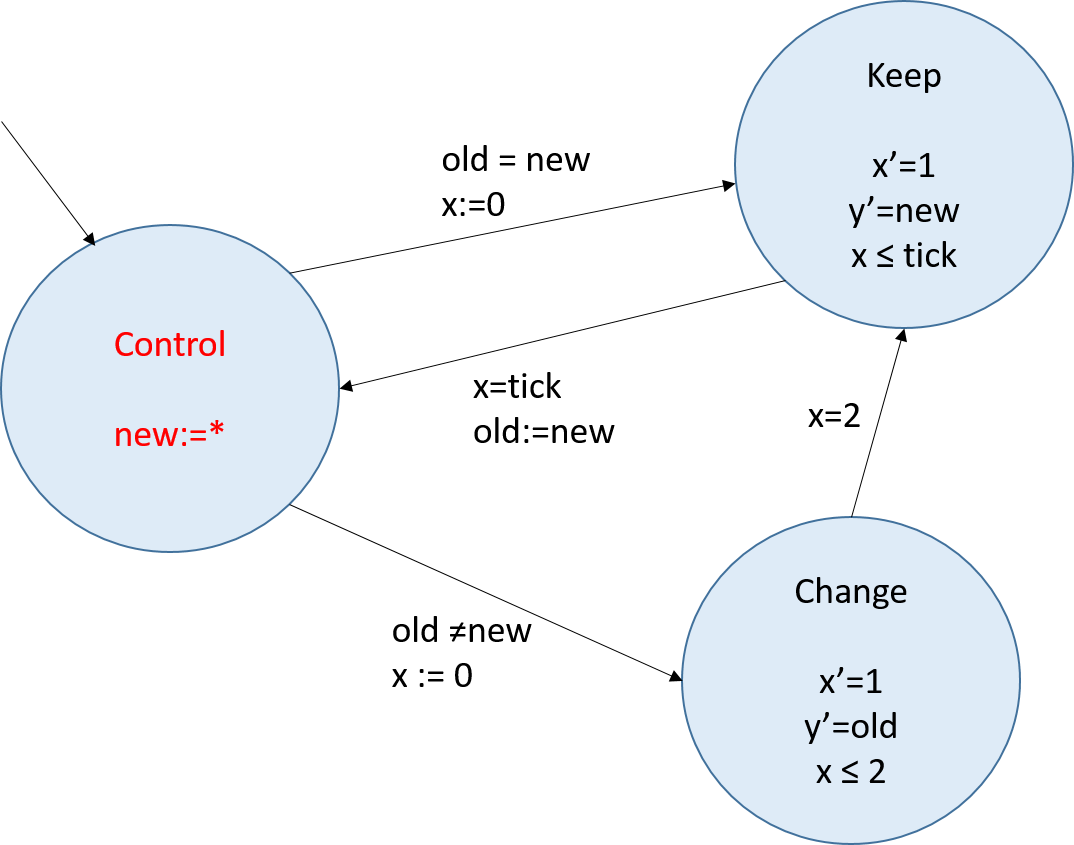
\includegraphics[height=0.5\textheight,width=0.8\textwidth]{Images/ha_control}
		\caption{Watertank Hybrid  Automata with Non-Deterministic Control Program Abstraction marked.}
		\label{fig:ex_control}
	\end{figure}

\section{Listings}
\label{app:sec:listings}

In the following section we present the full java source code for our control program classes, as well as the rule definition we used for \keym. First is the rule definition for \keym, that abstracts the application of the floor function to a inequality of the form \(\textrm{floor}(x) = y \equiv \exists c:x-1 < c \wedge c \leq x \wedge (x \geq 0 \implies c \geq 0) \wedge (x < 0 \implies c < 0)  \longrightarrow\) whereby \(\longrightarrow\) refers to the big implication arrow in the verification of a hybrid program, meaning we get the abstraction of \(f(x)\) on the left side of the implication.

\lstset{language=Java,captionpos=b,tabsize=3,frame=lines,keywordstyle=\color{black},commentstyle=\color{black},stringstyle=\color{black},numbers=left,numberstyle=\tiny,numbersep=5pt,breaklines=true,showstringspaces=false,basicstyle=\footnotesize,emph={label}}
\begin{lstlisting}[label=app:lst:ruleF]
	\rules {
 	 	fdef {
			\schemaVar \term R x;
			\schemaVar \skolemTerm R c;
    			\find(f(x))
			\sameUpdateLevel
			\varcond ( \new(c, \dependingOn(x)) )
			\replacewith(c)
			\add(x-1 < c & c <= x & (x >= 0 -> c >= 0) & (x < 0 -> c < 0) ==> )
			\heuristics(simplify)
		};
	}	
\end{lstlisting}

Next, we provide the full java source code for the Watertank control program class. This means, not only the control method itself is provided, but all the needed class definitions as well.

\lstset{language=Java,captionpos=b,tabsize=3,frame=lines,keywordstyle=\color{blue},commentstyle=\color{darkgreen},stringstyle=\color{red},numbers=left,numberstyle=\tiny,numbersep=5pt,breaklines=true,showstringspaces=false,basicstyle=\footnotesize,emph={label}}
\begin{lstlisting}[label=app:lst:watertankContr]
package watertankSplit;

/**
 * @author Daniel Draper
 * @version 1.0
 * This class is the Watertank's control system.
 */
public class Controller {
	private int tick;
	
	public Controller() {
		tick = 30;
	}
	
	/**
	 * Returns the actual control value for the valve of the watertank.
	 * @param y the current water level
	 * @param old the old valve setting
	 * @return the new valve setting
	 */
	/*@ public normal_behavior
	  @ requires tick == 31 && y >= 10 && y <= 120 && y + 2 * old <= 120 && y + 2 * old >= 10 && (old == 10 || old == -20);
	  @ ensures \result * (tick / 10) + y + 2 * old  >= 12 & \result * (tick / 10) + y + 2 * old <= 116 && (\result == 10 || \result == -20);
	  @*/
	public int getControlValue (int y, int old) {
		//Waterlevel in two time units
		int inTwo = y + 2 * old;
		//If we are raising level, keep raising if possible without hitting max_level before next tick
		if (old == 10) {
			if (inTwo + tick * 1 <= 116) {
				return 10;
			}
			else {
					return -20;
			}
		}
		//ELSE if we are currently lowering level, keep lowering if we can lower further without hitting min_level b4 next tick
		else {
			if (old == -20) {
				if (inTwo - tick * 2 >= 12) {
					return -20;
				}
				else {
						return 10;
				
				}
		
			}
		}
		//Only returned if old != 10 && old != -20, unreachable.
		return 0;
	}
}
\end{lstlisting}

Next, you can find the full source code for the Traffic Control Car Control Program. 

\begin{lstlisting}[label=app:lst:carContr]
package trafficControl;

/**
 * @author Daniel Draper
 * @version 1.0
 * This class models the Car Controller of the Traffic Control CPS.
 */
public class CarController {
	private int TICK;
	private int MAXBREAK;
	private int MAXACCEL;

	public CarController(int TICK, int MAXBREAK, int MAXACCEL) {
		this.TICK = TICK;
		this.MAXBREAK = MAXBREAK;
		this.MAXACCEL = MAXACCEL;
	}
	/**
	 * @param slPos Current Speed Limit Position
	 * @param sl current Speed Limit
	 * @param y current Car Position 
	 * @param v current Car Velocity
	 * @param accel current Car acceleration
	 * @return the new acceleration control Value
	 * The actual control Method.
	 */
	/*@ public normal_behavior
	  @ requires MAXBREAK <= accel && accel <= MAXACCEL && ((!(y >= slPos)) || v <= sl) && v >= 0 && sl >= 0 && TICK == 1 && MAXBREAK == -10 && MAXACCEL == 10 && 2 * MAXBREAK * (slPos - y) >= v*v - sl*sl && (v <= sl || slPos * 2 * MAXBREAK >= y*2*MAXBREAK + (v*v - sl*sl));
	  @ ensures MAXBREAK <= \result && \result <= MAXACCEL && ((!(y >= slPos)) || (\result*TICK <= (sl - v))) && ((!(y < slPos)) || (2*slPos*MAXBREAK*(-1) >= y*2*(-1)*MAXBREAK + (v*v - sl*sl)  + (\result+(-1)*MAXBREAK) * (\result * TICK*TICK + 2*TICK * v)));
	 @*/
	public int control(int y, int v, int accel, int sl, int slPos) {
		if (y >= slPos) {
			if ((accel+1)*TICK <= (sl-v)) {
				if (accel+1 <= MAXACCEL) {
					return accel+1;
				}
				
			}
			else {
				if((accel-1)*TICK <= (sl-v)) {
					if (accel-1 >= MAXBREAK) {
						return accel-1;
					}
			}
			}
		}
		else {
			if (2*slPos*MAXBREAK*(-1) >= y*2*(-1)*MAXBREAK + (v*v - sl*sl)  + ((accel+1)+(-1)*MAXBREAK) * ((accel+1) * TICK*TICK + 2*TICK * v)) {
				if (accel+1 <= MAXACCEL) {
					return accel+1;
				}
			}
			else {
				if (2*slPos*MAXBREAK*(-1) >= y*2*(-1)*MAXBREAK + (v*v - sl*sl)  + ((accel-1)+(-1)*MAXBREAK) * ((accel-1) * TICK*TICK + 2*TICK * v)) {
					if (accel-1 >= MAXBREAK) {
						return accel-1;
					}
				}
			}
		}
			return MAXBREAK;
		
	}
\end{lstlisting}

Next, you can find the full source code for the Speed Limit Control Class.
\begin{lstlisting}[label=app:lst:speed]

package trafficControl;


/**
 * @author Daniel Draper
 * @version 1.0
 * This class models the Speed Limit Controller used by the Traffic Control CPS.
 */
public class SpeedLimitController {

	private int TICK;
	private int MAXBREAK;
	private int MAXACCEL;
	/**
	 * @param TICK the Tick duration
	 * @param MAXBREAK the maximum breaking power (<0)
	 * @param MAXACCEL the maximum acceleration (>=0)
	 */
	public SpeedLimitController(int TICK, int MAXBREAK, int MAXACCEL) {
		this.TICK = TICK;
		this.MAXBREAK = MAXBREAK;
		this.MAXACCEL = MAXACCEL;
	}

	/**
	 * @param slPos the current speed limit position
	 * @param sl the current speed limit
	 * @param accel the current car's acceleration value
	 * @param v the current car's velocity
	 * @param y the current car's position
	 * @return both the new speed limit and speed limit position in an array.
	 * The actual control Method.
	 */
	/*@ public normal_behavior
	  @ requires MAXBREAK == -10 && MAXACCEL == 10 && TICK == 1 && ((!(y >= slPos)) || v <= sl) && v >= 0 && sl >= 0 && (v <= sl || slPos * 2 * MAXBREAK >= y*2*MAXBREAK + (v*v - sl*sl)) && ((!(sl < v)) || slPos * (-2) * MAXBREAK >= y*(-2)*MAXBREAK + (v*v - sl*sl) + (MAXACCEL + MAXBREAK) * (MAXACCEL * TICK*TICK + 2*TICK * v)) && ((!(sl >= v)) || accel*TICK <= (sl - v)) && (\exists int x;x>=0; (slPos+x) * (-2) * MAXBREAK >= y*(-2)*MAXBREAK + (v*v - sl*sl) + (MAXACCEL + (-1)*MAXBREAK) * (MAXACCEL * TICK*TICK + 2*TICK * v));
	  @ ensures \result[0] >= 0 && ((!(\result[0] < v)) || \result[1] * (-2) * MAXBREAK >= y*(-2)*MAXBREAK + (v*v - \result[0]*result[0]) + (MAXACCEL + (-1)*MAXBREAK) * (MAXACCEL * TICK*TICK + 2*TICK * v)) && ((!(\result[0] >= v)) || accel*TICK <= (\result[0] - v));
	*/
	public int[] control(int y, int v, int accel, int sl, int slPos) {
		int[] result = new int[2];
		result[0] = sl;
		result[1] = slPos;
		if (sl<25) {
			if (sl+1 < v) {
				result[0]++;
				result[1] = y + (v*v - result[0]) + (MAXACCEL  + 1) * (MAXACCEL * TICK*TICK + 2 * TICK * v);
			}
			else {
				if (accel*TICK <= result[0]+1 - v) {
					result[0]++;
				}
			}
		}
		else {
		if (result[0]-1 < v) {
			if (result[0]-1 >= 0) {
			result[0]--;
			
			result[1] = y + (v*v - result[0]) + (MAXACCEL  + 1) * (MAXACCEL * TICK*TICK + 2 * TICK * v);
			}
		}
		else {
			if (accel*TICK <= (result[0]-1 - v) && result[0]-1 >= 0) {
				result[0]--;
			}
		}
	}
		return result;

	}
}
\end{lstlisting}
\section{Watertank simulator}
\label{app:sec:simulator}

To be able to execute the watertank control programs and see a result of the computations done on screen (in a form of console output) we had to write a simulator of the differential evolution of the watertank values. The watertank simulator class can be found below:

\begin{lstlisting}[label=app:lst:watertankSim]
package watertankSplit;

/**
 * @author Daniel Draper
 * @version 1.0
 * This class simulates a watertank as modelled in the hybrid model in the KeYmaera Guide.
 */

public class Simulator
{
	private int TICK = 30;
	private Controller contr;
	private int y;
	private int x;
	private int state;
	private int oldDif;
	private int newDif;
	
	/**
	 * Constructs the simulator with correct starting values according to hybrid model.
	 */
	public Simulator() {
		contr = new Controller();
		state = 1;
		y = 10;
		x = TICK;
		oldDif = 10;
		newDif = 10;
	}
	
	/**
	 * One step in the differential evolution of the watertank.
	 */
	private void step() {
		switch (state) {
		case 0:
			if (x == 20) {
				state = 1;
			}
			else {
				y+=oldDif;
				x+=10;
			}
			break;
		case 1:
			if (x == TICK) {
				oldDif = newDif;
				System.out.println("Controlled!");
				newDif = contr.getControlValue(y, oldDif);
				if (newDif == oldDif) {
					state = 1;
					x = 0;
				}
				else {
					state = 0;
					x = 0;
				}
			}
			else {
				y+=newDif;
				x+=10;
			}
			break;
	}
	}
	
	/**
	 * Continuous execution of each timestep and printing the state with an included delay.
	 */
	public void run() {
		do {
			step();
			printState();
				synchronized(this) {		
					try {
						this.wait(500);
					} catch (InterruptedException e) {
						e.printStackTrace();
					}	
					finally {} 
				}
		} while(true);
	}
	/**
	 * Prints the current state of the Watertank.
	 */
	private void printState() {
		System.out.println("Time: " + x/10 + " newDif: " + newDif + " Fillstatus:");
		for (int i = 0; i < y/10; i++) {
		System.out.print("X ");
		}
		for (int i = 0; i < 12 - y/10; i++) {
			System.out.print("_ ");
		}
		System.out.println();
		
	}
	
	/**
	 * Main function creating and executing a new Simulator.
	 * @param args commandline arguments
	 */
	public static void main(String args[]) {
		Simulator s = new Simulator();
		s.run();
	}

}
\end{lstlisting}

\section{Traffic Control Simulator}
\label{app:sec:TrafficSim}

As we did for the Watertank CPS, we also wrote a Simulator for the Traffic Control CPS as to be able to execute the entire program and see the evolution of the car. As the amount of distance between the next speed limit and current car's position can vary greatly, we chose a different way to present the current status of the system than for the watertank, just listing the current status in text form and checking if safety is still guaranteed. It consists of an infinite loop always continuing with one step in the differential evolution of the system, printing the state and an added delay as to make console output readable.

\begin{lstlisting}[label=app:lst:trafficSim]

package trafficControl;

/**
 * @author Daniel Draper
 * @version 1.0
 * This class simulates the environment in the Traffic Control CPS.
 */
public class Simulator {

	private int xDif;
	private int x;
	private int y;
	private int v;
	private int accel;
	private int sl;
	private int slPos;
	private CarController carContr;
	private SpeedLimitController limContr;
	private static int TICK = 1;
	private static int MAXACCEL = 10;
	private static int MAXBREAK = -10;
	
	/**
	 * Creates a new Traffic Control Simulator.
	 */
	public Simulator() {
		xDif = 1;
		v = 10;
		x = 0;
		y = 0;
		slPos = 10;
		sl = 10;
		carContr = new CarController(TICK, MAXBREAK, MAXACCEL);
		limContr = new SpeedLimitController(TICK,MAXBREAK,MAXACCEL);
	}
	
	/**
	 * Starts the entire system, running in an infinite loop.
	 */
	public void run() {
		do {
			printState();
			if (x \% TICK == 0) {
				accel = carContr.control(y,v,accel,sl,slPos);
					int[] res = limContr.control(y,v,accel,sl,slPos);
					sl = res[0];
					slPos = res[1];
			}
			int v0 = v;
			x += xDif;
			v += accel;
			y += (v0 + 0.5 * accel);
				synchronized(this) {		
			try {
				this.wait(500);
			} catch (InterruptedException e) {
				// TODO Auto-generated catch block
				e.printStackTrace();
			}	
			finally {} 
		}
		} while(true);
	}
	/**
	 * Prints the current state of the system.
	 */
	private void printState() {
		System.out.println("We have: Car at Pos. " + y + " with velocity " + v + " and acceleration " + accel);
		System.out.println("Speed limit " + sl + " at Pos. " + slPos);
		System.out.println("If car breaks at max_Break_Speed " + MAXBREAK + " at next tick, car has speed " + (v + accel) + " and afterwards speed " + (v+accel+MAXBREAK));
		if (y >= slPos) {
			if (accel*TICK <= (sl- v)) {
				System.out.println("Safety kept!");
				return;
			}
		}
		else {
			if (2*slPos*MAXBREAK*(-1) >= y*2*(-1)*MAXBREAK + (v*v - sl*sl)  + (accel+(-1)*MAXBREAK) * (accel * TICK*TICK + 2*TICK * v)); {
				System.out.println("Safety kept!");
				return;
			}
		}
		System.err.println("Safety condition not kept!");
	}

	/**
	 * @param args Commandline Arguments.
	 * Main function for execution.
	 */
	public static void main(String[] args) {
		Simulator s = new Simulator();
		s.run();
	}
}
\end{lstlisting}

\section{Complete Hybrid Programs in correct ASCII notation}
\label{app:sec:pdfs}

In this section we present the complete hybrid programs from this thesis. As we mentioned in Ch.~\ref{ch:Preliminary}, hybrid programs have to be typeset in ASCII for \keym~to be able to read it, which is why these hybrid programs look different from the ones we present in the previous chapters. The first two hybrid programs are the original watertank hybrid program and our remodelled version that includes the hook, a suitable postcondition as well as the tick.
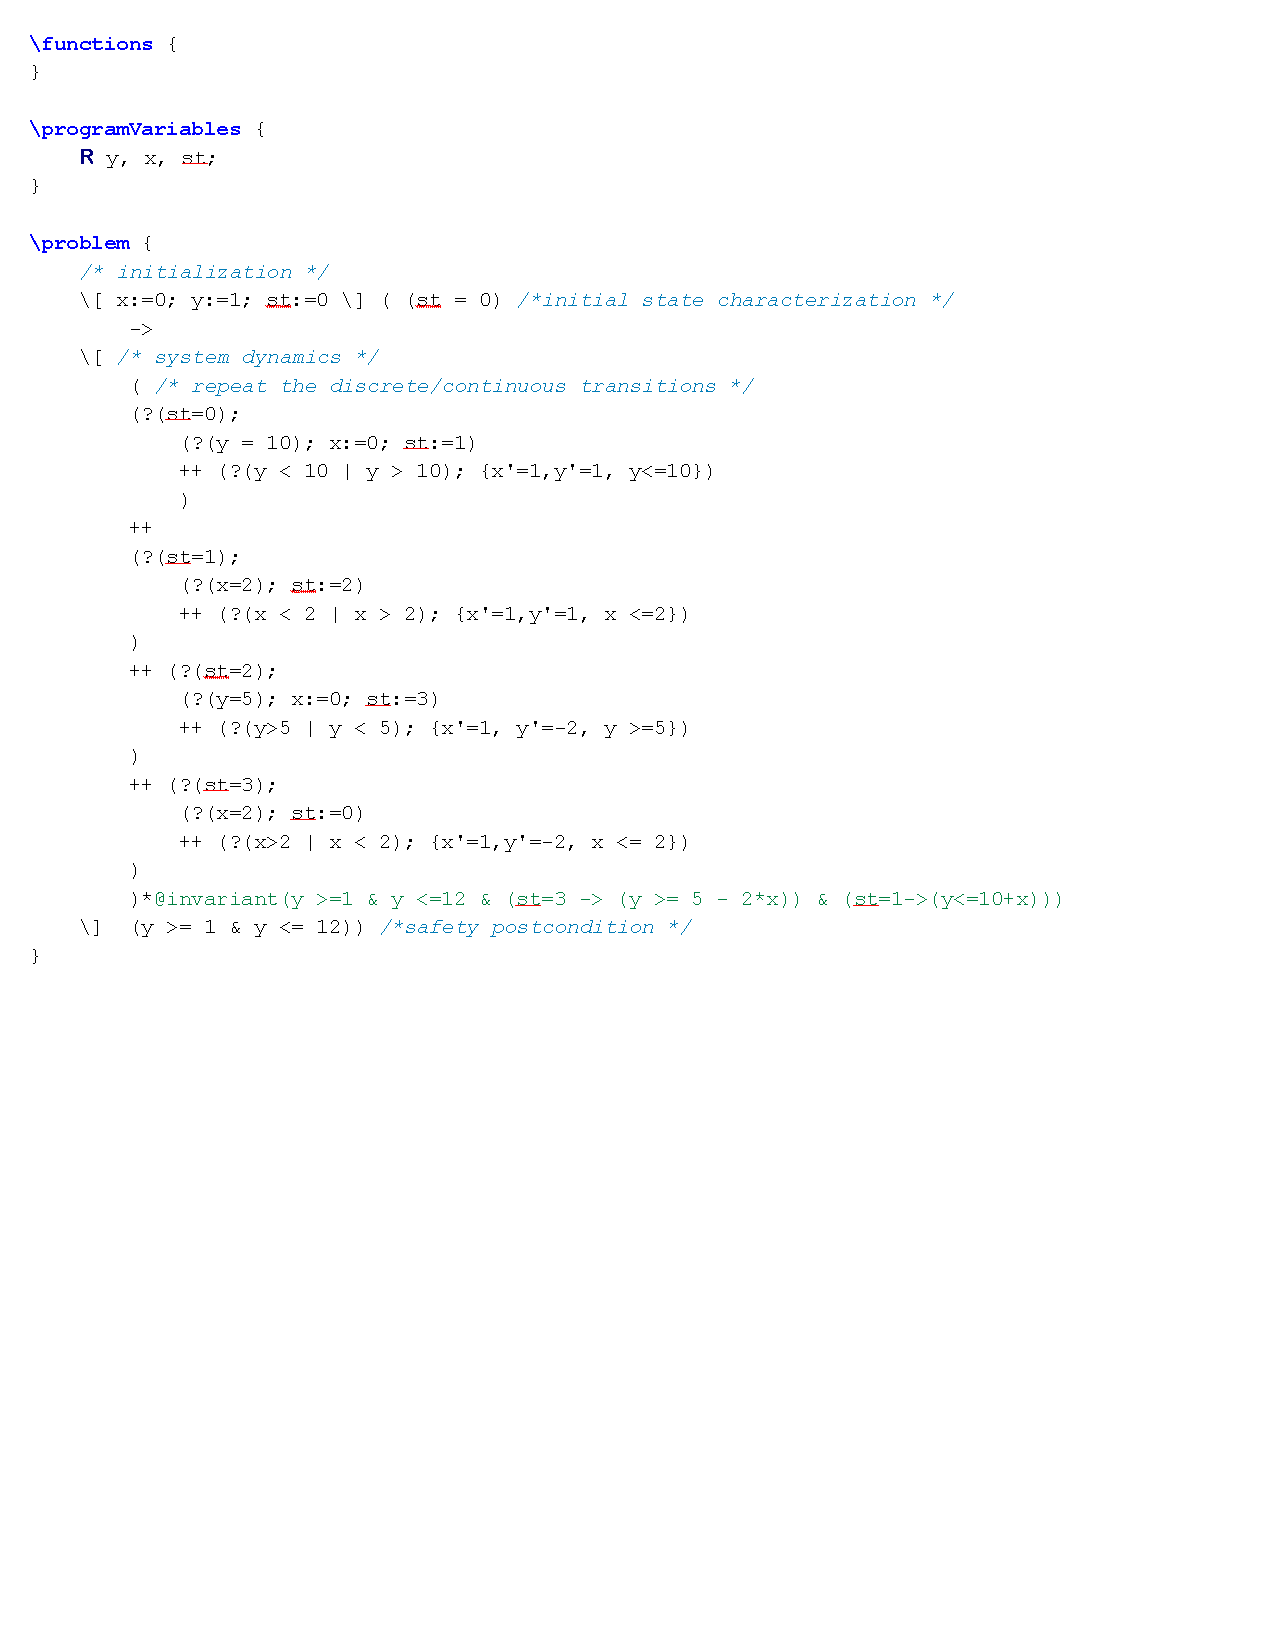
\includepdf[pages=1,scale=1]{images/watertank_hp.pdf}

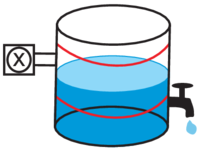
\includepdf[pages=1,scale=1]{images/watertank.pdf}

Next up is the glue proof for the watertank cps typeset in ASCII.

\includepdf[pages=1,scale=1]{images/glue.pdf}

The next two hybrid programs are the original Traffic Control hybrid program, as well as it's remodelled version that includes the hooks (as in this case we have two control programs), the postconditions and a tick.
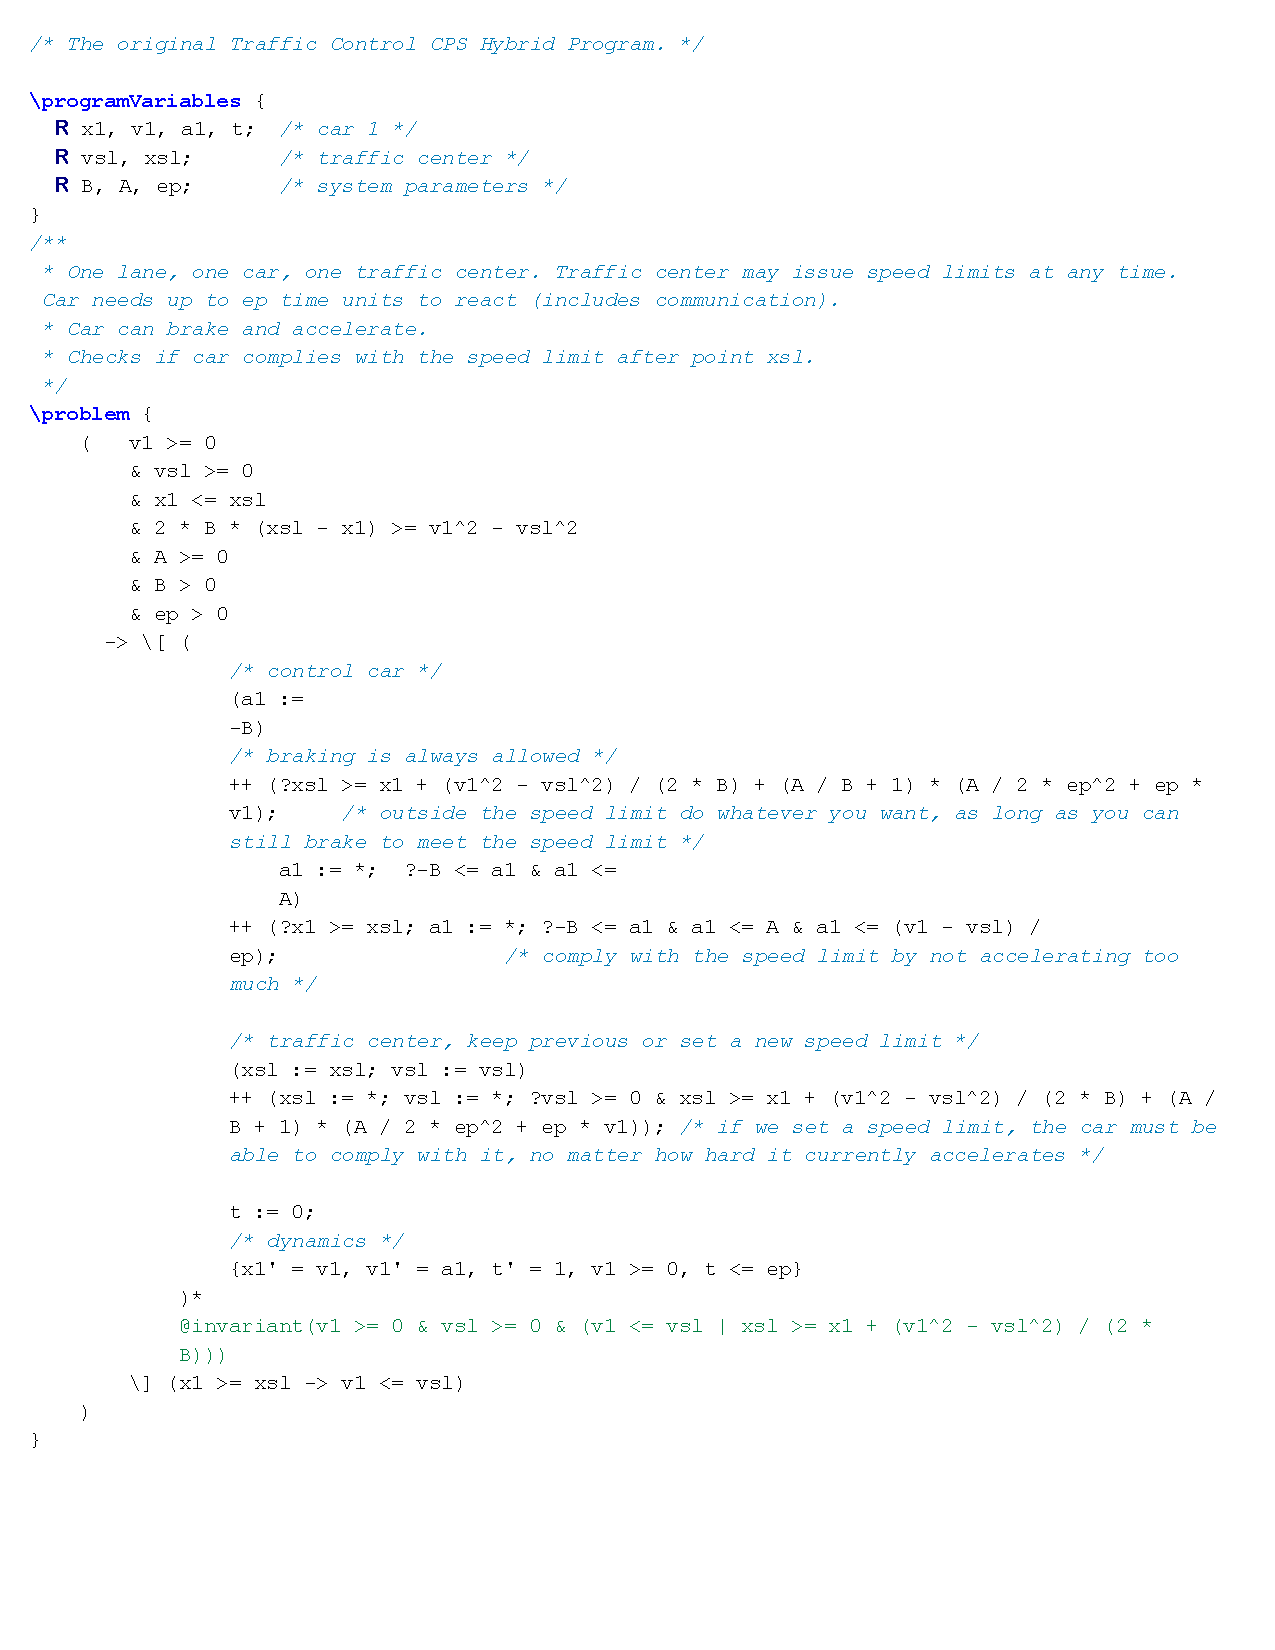
\includepdf[page=1,scale=1]{images/trafficControlOrig.pdf}

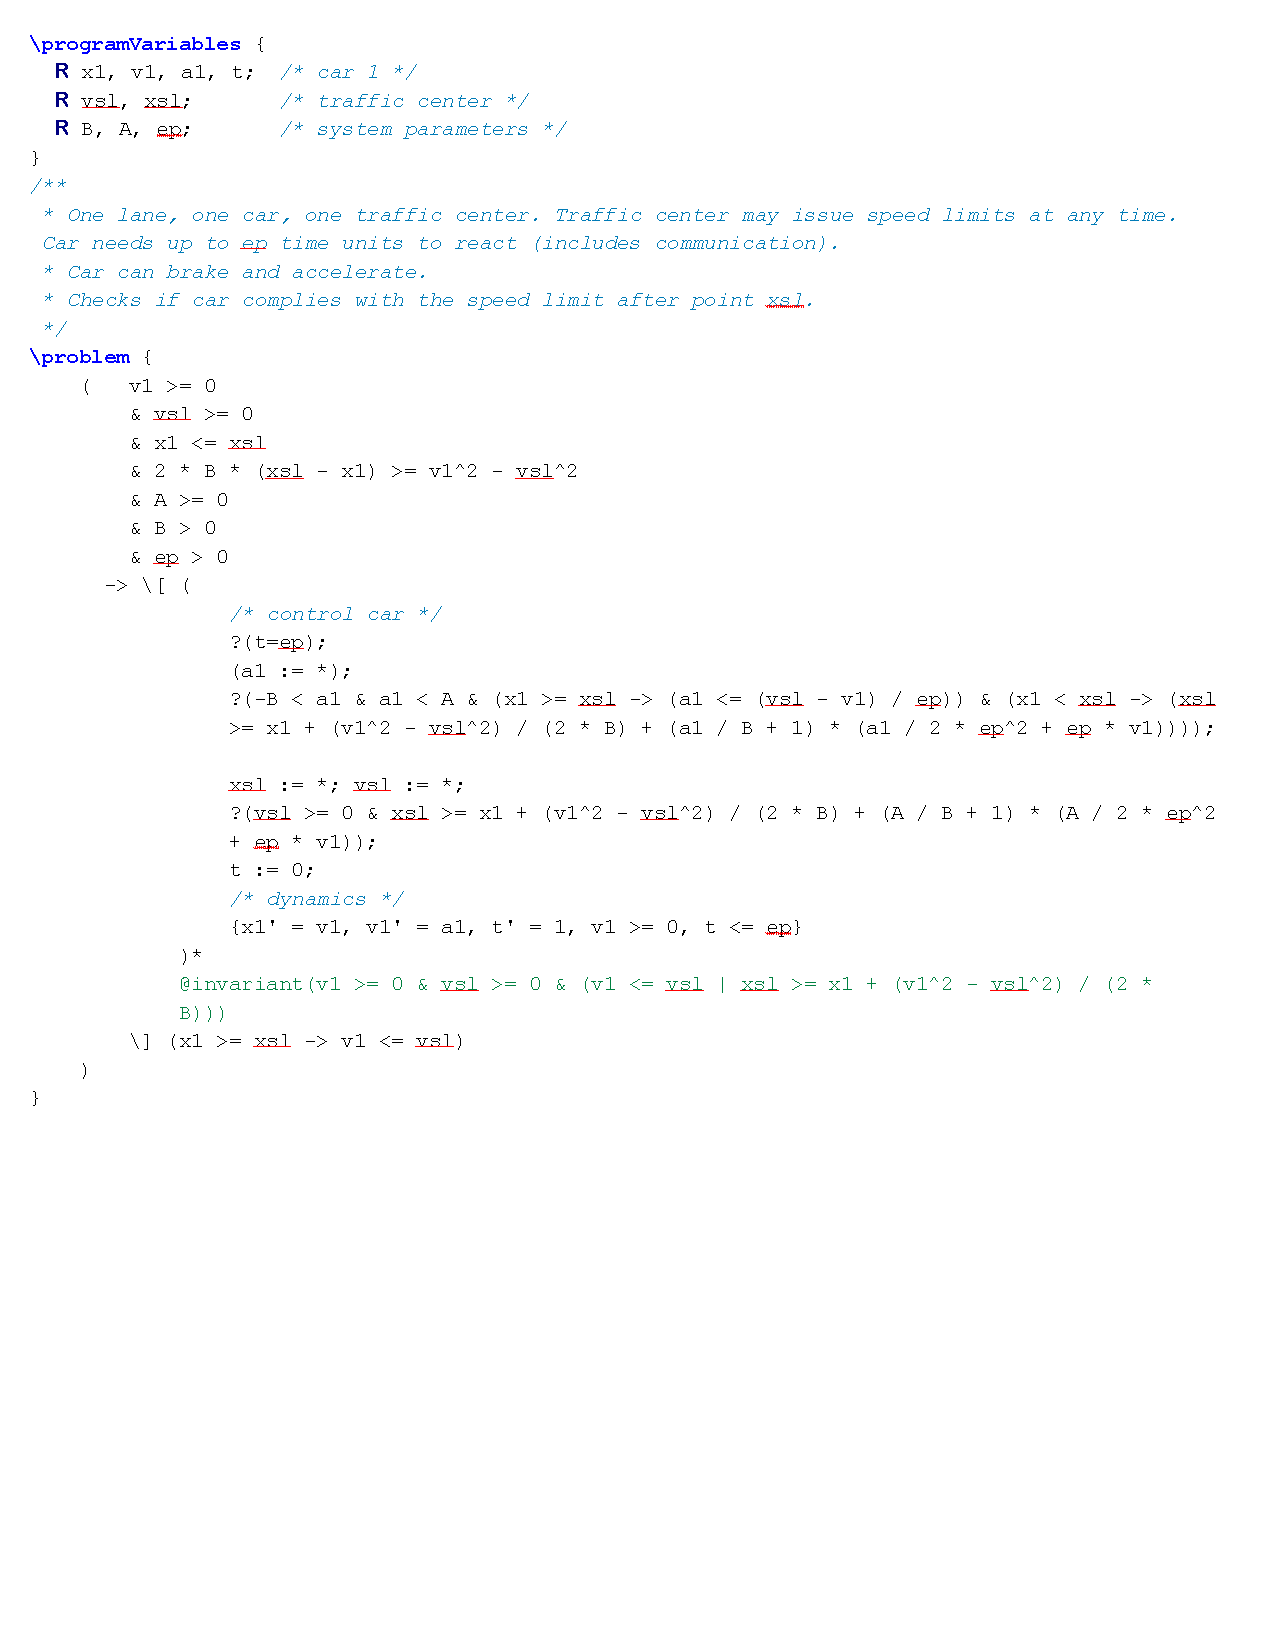
\includepdf[page=1,scale=1]{images/trafficControlRem.pdf}

What now follows is the glue proof for the traffic control cps typeset in ASCII.


\newglossaryentry{cps} {
 name=Cyber-Physical System[CPS],
 description={is a system describing motions or evolutions in which a physical aspect is being controlled by a computer/computer program. In this thesis equivalent to the notion of Hybrid Systems.}
}

\newglossaryentry{hybrid}{
 name=Hybrid System,
 description={is a system in which discrete as well as continuous evolutions are present. E.g, a remote controlled car which can only be accelerated or braked, its movement is continuous and follows continuous differential equations, while the control program is discrete and can only take discrete values (e.g, Acceleration := 1; Acceleration := 2 etc.).}
}

\newglossaryentry{hook}{
name=Hook,
description={refers to a/multiple concrete instruction at which the control program is executed when describing a hybrid system as a hybrid program. This is one or multiple non-deterministic assignments of values, e.g a:=*.}
}

\newglossaryentry{hookcond}{
name=Hook Safety Postcondition,
description={refers to the condition that has to be fullfilled by the value(s) that were assigned in the hook for the safey condition of the whole program to hold true.}
}

\newglossaryentry{glue}{
name=Glue,
description={refers to a relation between the values in the world of reals and the discrete world. For us, refers to a way of gaining the corresponding value in the other world from a given value.}
}

\newglossaryentry{hybridProg}{
name=Hybrid Program,
description={is a way to describe hybrid systems in the form of a program. Expressed in the syntax of regular programs with the extension of differential equations.}
}

\newglossaryentry{hybridAuto}{
name=Hybrid Automata,
description={is a way to model hybrid systems in the form of a non-deterministic automata. Uses the same syntax as finite automata with the addition of differential equations.}
}

\newglossaryentry{dl}{
name=Dynamic Logic,
description={is the logic we use to express the safety property for our CPS.}
}

\newglossaryentry{DDL}{
name=Differntial Dynamic Logic[DDL],
description={is the logic in which we express the safety properties for our CPS, and it also includes a syntax to express differential equations.}
}

\newglossaryentry{key}{
name=\key,
description={is the tool we use to verify our java control programs as our concrete implementations.}
}

\newglossaryentry{keym}{
name=\keym,
description={is the tool we use to verify both our remodelled hybrid programs as well as the glue relation.}
}

\newglossaryentry{jml}{
name=Java Modelling Language,
description={is the language we use to express the contracts a certain method or class has to fulfill to be considered correct.}
}




\end{document}
